\section{The Data}
\label{sec:data}

We used the Kepler-Gaia cross-matched catalog available at gaia-kepler.fun,
which includes 194764 Kepler targets, cross-matched with Gaia targets within
in a 1'' radius.
This catalog includes Gaia positions, parallaxes, and proper motions from
Gaia EDR3 and RVs from Gaia DR2.
It also includes distances inferred from Gaia EDR3 parallaxes
\citep{bailer-jones2021}.
% created using the cross-match service and Vizier catalogue access tool
% provided by CDS, Strasbourg, France, as well as the astroquery and astropy
% python packages.
We crossmatched this catalog with the LAMOST DR5 catalog, also using a 1''
radius and, where available, added APOGEE RVs from the DR16 stellar catalog
\citep{apogee_dr16}.
We removed stars with a Gaia parallax $<$ 0, parallax signal-to-noise ratio
$<$ 10, or Gaia astrometric excess noise $>$ 5.
After applying these cuts our total number of targets was \nstars\ stars:
\ngaia\ with RVs from Gaia DR2, \nlamost\ from LAMOST DR5, and \napogee\ from
APOGEE DR16.
In total, \nrv\ stars in our sample have RVs from {\it either} Gaia, LAMOST,
or APOGEE.
The APOGEE survey has a higher spectral resolution than Gaia, which in turn is
higher than LAMOST.
The median RV uncertainty for stars in our sample is around 0.1 km/s for
APOGEE RVs, 1 km/s for Gaia RVS, and 4 km/s for LAMOST RVs.
In cases where stars had two or more available RV measurements, we adopted
APOGEE RVs as a first priority, followed by Gaia, then LAMOST.

Although RVs are available for more than one in three stars in this \kepler\
sample, most stars with RVs are bright.
Very few of the faintest stars have RV measurements because of the selection
functions of spectroscopic surveys.
% In our sample, one in 2.5 stars hotter than 5000 K had RV measurements,
% whereas only one in six stars cooler than 5000 K had RVs.
Most of the stars in our sample with Gaia RV measurements are brighter than
around 14th magnitude in Gaia $G$-band, and stars with LAMOST or APOGEE RVs
are mostly brighter than around 16th magnitude.
Figure \ref{fig:rv_histogram} shows the apparent magnitude and temperature
distributions of the stars in our sample, with and without RVs.
This figure reveals the combined selection functions of the Gaia, LAMOST and
APOGEE RV surveys and shows that faint stars have fewer RV measurements than
bright ones.
\begin{figure}[ht!]
\caption{
    % The apparent magnitude (left) and temperature (right) distributions of
    % stars in our sample, with and without RV measurements from \gaia\ and
    % \lamost.
    The distribution of apparent Gaia magnitudes for
    stars in our sample with and without RV measurements from Gaia, LAMOST and
    APOGEE.
}
  \centering 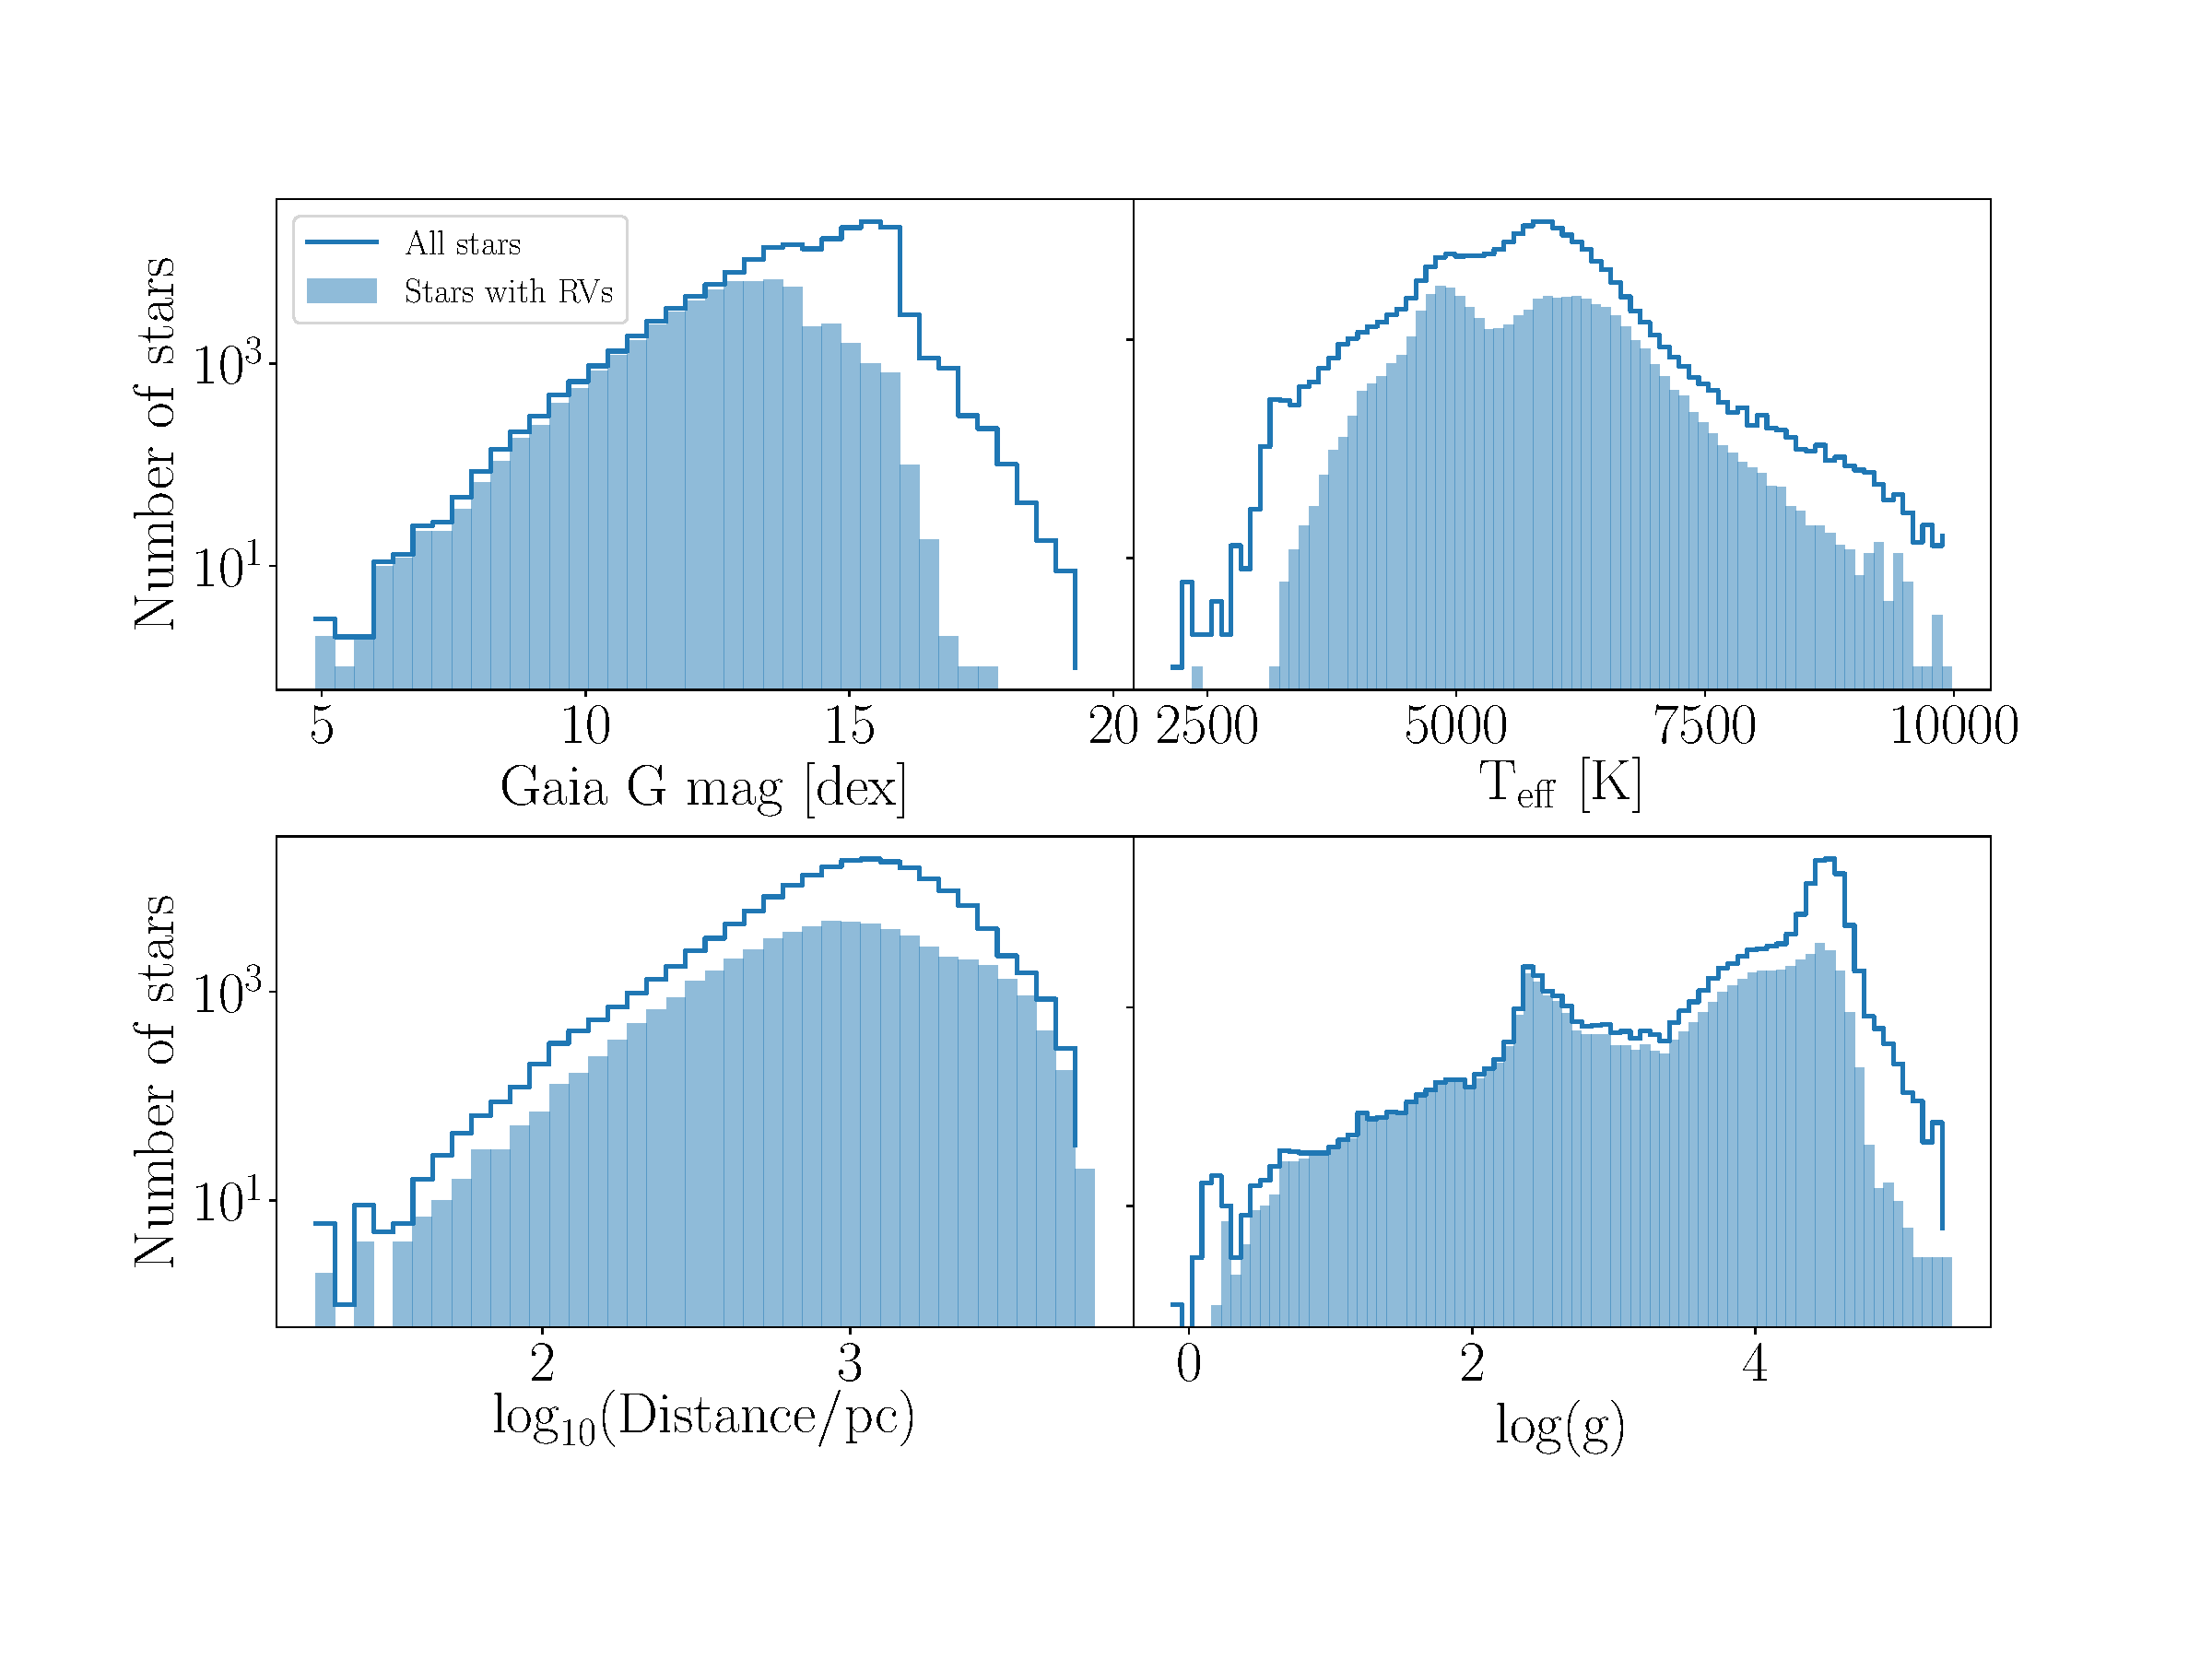
\includegraphics[width=.5\textwidth]{rv_histogram}
\label{fig:rv_histogram}
\end{figure}

To illustrate how the populations of stars with and without RVs differ, we
plot them on a color-magnitude diagram (CMD) in figure \ref{fig:CMD}.
The stars with RVs are generally hotter and more luminous than stars without.
Most stars with RVs fall on the upper main sequence, the red giant branch, and
the red clump.
Most stars without RVs fall on the main sequence.
This overall selection function is a combination of the APOGEE, LAMOST and
Gaia DR2 selection functions.
% The Gaia DR2 selection function is primarily a cut in apparent Gaia $G$-band
% magnitude.
% The LAMOST selection function is...
% The APOGEE selection function is...
\begin{figure}[ht!]
\caption{
    The color-temperature diagram of stars in the Kepler field with (left)
    and without (right) RVs provided by Gaia, LAMOST and APOGEE.
    The stars with RVs are generally hotter and more luminous than those
    without RVs, and include a large number of red clump stars and red giant
    branch stars.
    Stars without RVs are mostly concentrated on the main sequence.
}
  \centering 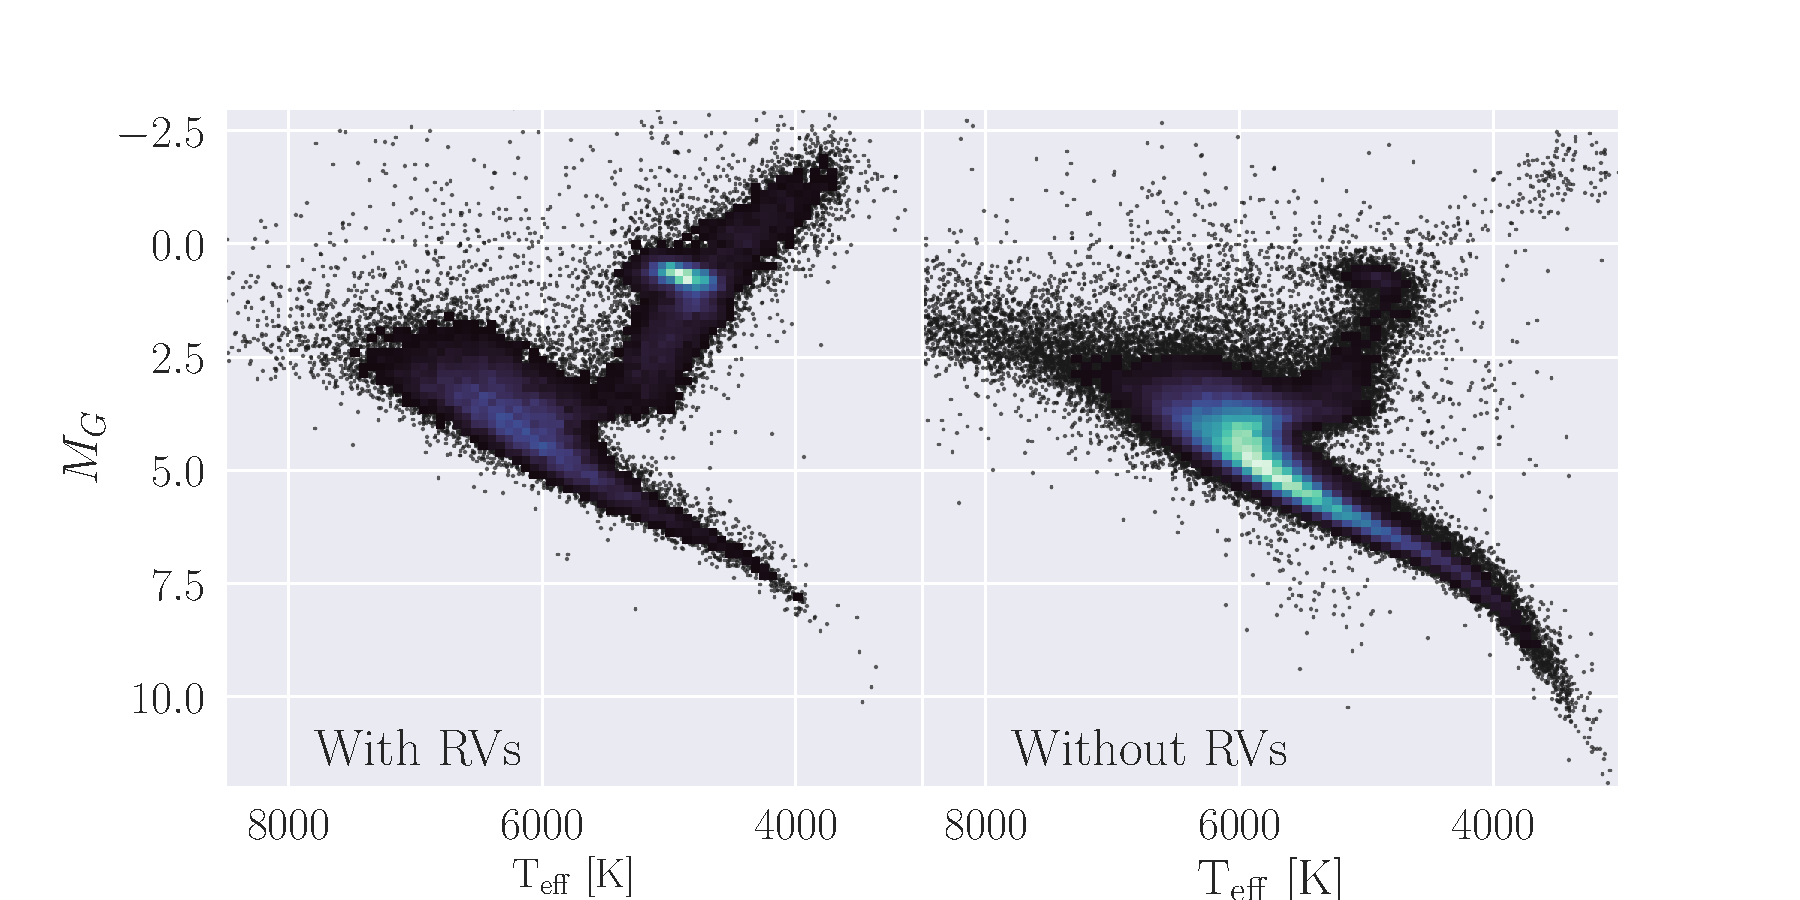
\includegraphics[width=1\textwidth]{CMD}
\label{fig:CMD}
\end{figure}
